\chapter{Kết quả thực nghiệm}
\label{chap:results}

Chương này tách rõ bằng chứng thăm dò lịch sử khỏi kết quả xác nhận chính. Kết
quả chính bên dưới được tính từ hai tập Test-100 sau khi policy đã được đóng
băng. Các bảng đầy đủ gồm toàn bộ 14 policy, kể cả những policy không nằm trên
đường Pareto, nhằm tránh chỉ báo cáo các cấu hình thuận lợi.

\section{Bằng chứng thăm dò từ mô hình 1.7B}

Thực nghiệm Qwen3-1.7B trước khi chốt protocol chính dùng GSM8K và revision có
tiền tố \code{70d244cc}. Manifest chứa 100 câu, trong đó 99 câu dùng được cho
phân tích định lượng; toàn bộ lưới có 1\,200 bản ghi. Hình
\ref{fig:historical-heatmap} cho thấy accuracy tăng khi tăng cả $k$ và $L$,
đồng thời mức cải thiện theo depth nổi bật trong cấu hình pilot. Quan sát này
chỉ tạo giả thuyết và đã được dùng để thiết kế protocol 0.6B; nó không được gộp
với Test chính và không được xem là bằng chứng xác nhận cho Research Question.

\begin{figure}[htbp]
  \centering
  \includegraphics[width=0.72\textwidth]{accuracy_heatmap.png}
  \caption{Heatmap accuracy của thực nghiệm lịch sử Qwen3-1.7B trên 99 câu
  GSM8K dùng được. Tiêu đề ``pilot items'' trong hình phản ánh đúng vai trò
  thăm dò của artifact gốc.}
  \label{fig:historical-heatmap}
\end{figure}

\section{Kết quả chính trên hai tập Test}

Bảng~\ref{tab:primary-test-results} trình bày các điểm vận hành cần thiết để
trả lời câu hỏi nghiên cứu. ``Selected'' là policy được chọn trên Validation
trước khi đọc Test; các comparator fixed và adaptive còn lại được lấy từ cùng
registry đã đóng băng.

% Generated by scripts/build_thesis_results.py. Do not edit manually.
\begin{table}[htbp]
  \centering
  \caption{Các điểm vận hành chính trên hai tập Test đóng băng. Khoảng tin cậy là Wilson 95\%.}
  \label{tab:primary-test-results}
  \scriptsize
  \begin{tabular}{p{0.12\textwidth}p{0.34\textwidth}rrr c}
    \toprule
    Dữ liệu & Policy & Đúng & Wilson CI (\%) & Token TB & Pareto \\
    \midrule
GSM8K & Breadth stop, $L=1024$ (selected) & 76/100 & [66.8, 83.3] & 1\,994.52 & Có \\
GSM8K & Joint heuristic & 70/100 & [60.4, 78.1] & 1\,449.46 & Có \\
GSM8K & Fixed $k=4,L=1024$ & 76/100 & [66.8, 83.3] & 2\,535.17 & Không \\
MATH-500 & Fixed $k=2,L=4096$ (selected) & 66/100 & [56.3, 74.5] & 5\,141.50 & Có \\
MATH-500 & Joint heuristic & 36/100 & [27.3, 45.8] & 5\,788.81 & Không \\
MATH-500 & Breadth stop, $L=4096$ & 73/100 & [63.6, 80.7] & 8\,191.12 & Có \\
MATH-500 & Fixed $k=4,L=4096$ & 73/100 & [63.6, 80.7] & 10\,233.17 & Không \\
    \bottomrule
  \end{tabular}
\end{table}


Hình~\ref{fig:cross-dataset-pareto} biểu diễn toàn bộ 14 policy của mỗi bộ dữ
liệu trong không gian accuracy--token. Vòng tròn đen đánh dấu policy selected;
đường nét đứt chỉ đường biên Pareto mô tả. Hình được sinh từ summary Test chính
và có dữ liệu thật, không phải khung giữ chỗ.

\begin{figure}[htbp]
  \centering
  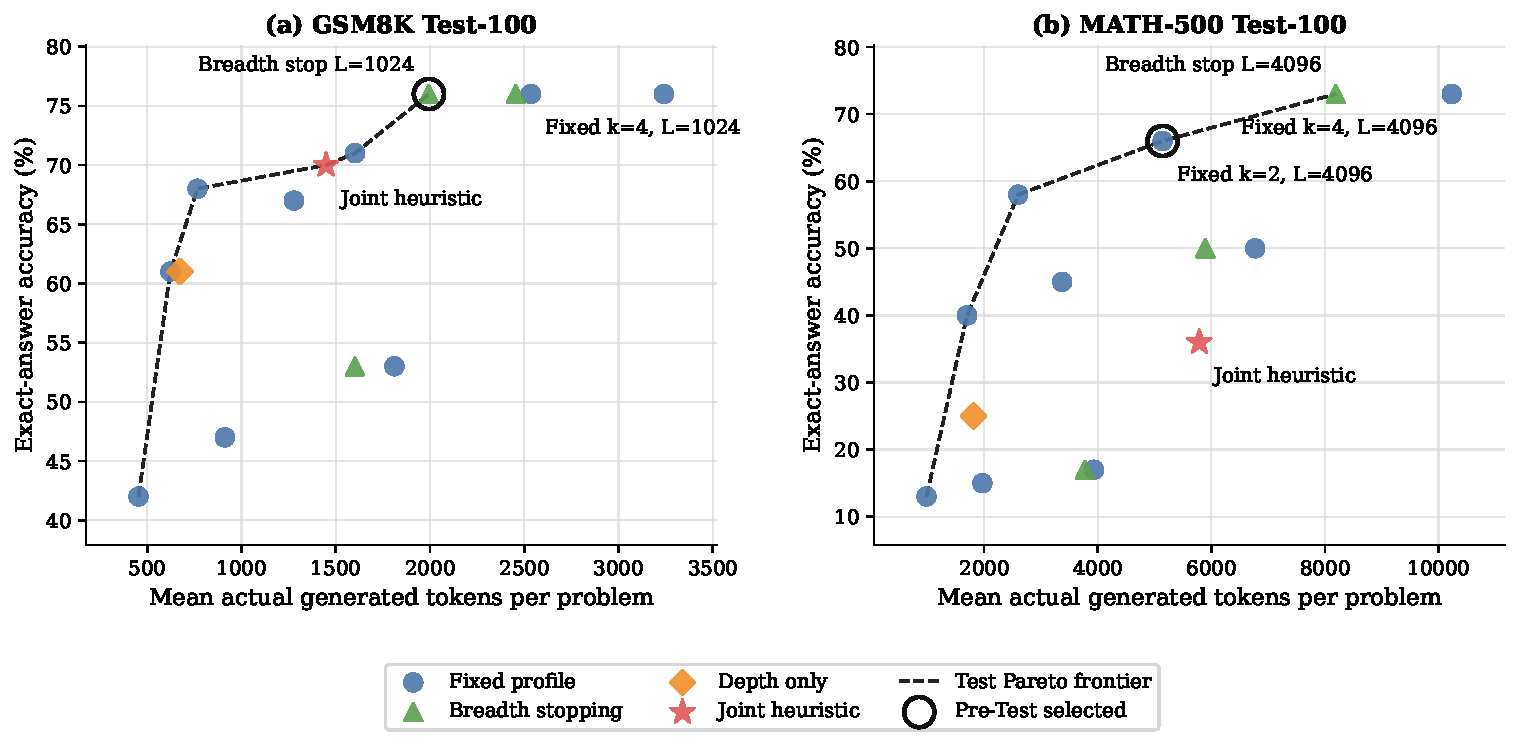
\includegraphics[width=\textwidth]{cross_dataset_test_policy_pareto.pdf}
  \caption{Accuracy và chi phí token của 14 policy đã đăng ký trên GSM8K và
  MATH-500 Test. Policy selected được quyết định trên Validation.}
  \label{fig:cross-dataset-pareto}
\end{figure}

\section{GSM8K: dừng breadth giữ nguyên độ chính xác với chi phí thấp hơn}

Policy selected breadth-only tại $L=1024$ đạt 76/100, khoảng Wilson 95\%
$[66.8,83.3]$, với 1\,994.52 token mỗi câu. Policy fixed $k=4,L=1024$ cũng
đạt 76/100 nhưng tốn 2\,535.17 token. Hai policy đúng và sai trên chính xác
cùng các câu Test (discordant 0/0), trong khi breadth stopping giảm 540.65
token, tương đương 21.33\% chi phí token. Policy dừng sau hai mẫu ở 54/100 câu
và dùng bốn mẫu ở 46/100 câu. Đây là bằng chứng trực tiếp rằng dừng theo đồng
thuận có thể loại bỏ mẫu dư thừa trong pool đã sinh mà không giảm accuracy ở
Test này.

Joint heuristic đạt 70/100 với 1\,449.46 token. So với joint, policy selected
tăng 6 điểm phần trăm nhưng trả thêm 545.06 token. Bảng ghép cặp có 7 câu chỉ
selected đúng và 1 câu chỉ joint đúng; McNemar exact cho $p=0.0703$, và
$p_{\mathrm{Holm}}=0.4922$. Vì vậy dữ liệu chưa đủ để khẳng định khác biệt
accuracy có ý nghĩa thống kê, dù hai điểm vận hành tạo ra đánh đổi chi phí--độ
chính xác khác nhau.

\section{MATH-500: joint heuristic không chuyển giao ổn định}

Policy selected fixed $k=2,L=4096$ đạt 66/100, khoảng Wilson 95\%
$[56.3,74.5]$, với 5\,141.50 token. Joint heuristic chỉ đạt 36/100 và tốn
5\,788.81 token; do đó bị trội cả về accuracy lẫn token. So sánh ghép cặp có
33 câu chỉ selected đúng và 3 câu chỉ joint đúng. McNemar exact cho
$p=2.27\times10^{-7}$ và sau điều chỉnh Holm còn
$p_{\mathrm{Holm}}=2.50\times10^{-6}$. Kết quả này bác bỏ việc xem joint
heuristic hiện tại là controller đa dữ liệu đã thành công.

Comparator breadth-only tại $L=4096$ đạt 73/100 với 8\,191.12 token, bằng
accuracy của fixed $k=4,L=4096$ nhưng thấp hơn 2\,042.05 token, tương đương
19.96\%. Hai policy một lần nữa có discordant 0/0. Breadth policy dừng ở hai
mẫu cho 57 câu và dùng bốn mẫu cho 43 câu. Kết quả này lặp lại lợi ích loại bỏ
sampling dư thừa, nhưng tại một điểm vận hành tốn chi phí hơn policy selected
và có accuracy cao hơn 7 điểm; luận văn không diễn giải chênh lệch đó như một
so sánh đã được chọn trước giữa hai policy.

\section{Phân tích ghép cặp}

Bảng~\ref{tab:paired-policy-results} tổng hợp các so sánh chính. Chênh lệch
token âm nghĩa là policy đứng trước rẻ hơn. Với các cặp breadth--fixed có
discordant 0/0, $p=1$ phản ánh không có khác biệt accuracy quan sát được; bằng
chứng hữu ích nằm ở phần giảm chi phí trên cùng vector đúng--sai.

% Generated by scripts/build_thesis_results.py. Do not edit manually.
\begin{table}[htbp]
  \centering
  \caption{So sánh ghép cặp chính. Chênh lệch được tính theo policy đứng trước trừ policy đứng sau; cột discordant là trước-only/sau-only.}
  \label{tab:paired-policy-results}
  \scriptsize
  \begin{tabular}{p{0.09\textwidth}p{0.24\textwidth}*{5}{>{\centering\arraybackslash}p{0.09\textwidth}}}
    \toprule
    Dữ liệu & So sánh & $\Delta$acc. (điểm) & $\Delta$token & Discordant & Exact $p$ & Holm $p$ \\
    \midrule
GSM8K & Selected vs joint & +6 & 545.06 & 7/1 & 0.0703 & 0.4922 \\
GSM8K & Breadth stop vs fixed $k=4$ & +0 & -540.65 & 0/0 & 1.0000 & -- \\
MATH-500 & Selected vs joint & +30 & -647.31 & 33/3 & $2.27\times10^{-7}$ & $2.50\times10^{-6}$ \\
MATH-500 & Breadth stop vs fixed $k=4$ & +0 & -2\,042.05 & 0/0 & 1.0000 & -- \\
    \bottomrule
  \end{tabular}
\end{table}


Kết quả trả lời revised RQ theo hai phần. Thứ nhất, adaptive breadth tạo ra
điểm vận hành chi phối comparator fixed-$k=4$ tương ứng trên cả hai dữ liệu.
Thứ hai, heuristic joint dựa trên độ dài prompt không đủ ổn định: nó vẫn nằm
trên Pareto GSM8K nhưng bị dominated rõ rệt trên MATH-500. Do đó đóng góp thực
nghiệm hiện tại là giao thức đánh giá và bằng chứng về breadth stopping, không
phải một learned joint controller hoàn chỉnh.

\section{Đối chứng non-thinking trên Validation}

Sau khi hoàn tất đánh giá Test chính, nghiên cứu thực hiện một đối chứng bổ
sung trên cùng 20 câu Validation của mỗi bộ dữ liệu. Hai chế độ dùng cùng
model revision, problem ID, prompt, sampling setting và các giá trị $k$; chỉ
thay đổi chế độ thinking. GSM8K dùng $L=2048$ và cùng parser V4 cho cả hai chế
độ, còn MATH-500 dùng $L=4096$ và parser V2. Không có artifact Test-100 nào
được mở để chọn hoặc đánh giá đối chứng này.

\begin{table}[htbp]
  \centering
  \caption{So sánh ghép cặp thinking và non-thinking trên Validation-20. Token
  là trung bình số token sinh thực tế trên mỗi câu.}
  \label{tab:nonthinking-validation}
  \scriptsize
  \begin{tabular}{llrrr}
    \toprule
    Dữ liệu & $(k,L)$ & Thinking: đúng/token & Non-thinking: đúng/token & Tiết kiệm token \\
    \midrule
    GSM8K & $(1,2048)$ & 13/20; 986.15 & 1/20; 31.30 & 96.83\% \\
    GSM8K & $(2,2048)$ & 14/20; 1\,969.70 & 1/20; 84.85 & 95.69\% \\
    GSM8K & $(4,2048)$ & 15/20; 3\,593.85 & 1/20; 143.65 & 96.00\% \\
    MATH-500 & $(1,4096)$ & 11/20; 2\,388.70 & 8/20; 471.90 & 80.24\% \\
    MATH-500 & $(2,4096)$ & 13/20; 4\,700.50 & 8/20; 923.40 & 80.36\% \\
    MATH-500 & $(4,4096)$ & 13/20; 8\,979.10 & 11/20; 1\,972.50 & 78.03\% \\
    \bottomrule
  \end{tabular}
\end{table}

Non-thinking giảm 78.03--96.83\% token nhưng có accuracy thấp hơn ở cả sáu
điểm. Trên GSM8K, chênh lệch là $-60$ đến $-70$ điểm phần trăm và cả ba kiểm
định McNemar vẫn có ý nghĩa sau hiệu chỉnh Holm
($p_{\mathrm{Holm}}\leq0.0004883$). Trên MATH-500, chênh lệch là $-10$ đến
$-25$ điểm; các kiểm định không có ý nghĩa tại $n=20$, điều này không chứng
minh tương đương hoặc non-inferiority. Vì cấu hình non-thinking rẻ nhưng không
giữ accuracy, nó không được đưa lên Test-100. Kết quả này là bằng chứng phát
triển bổ sung và không thay đổi các kết luận Test chính ở trên.

\section{Đối chứng maximum-budget force-answer}

Đối chứng thứ hai kiểm tra trực tiếp artifact do hard cap: dành $R=128$ token
trả lời trong tổng cap $L=512$ trên GSM8K và $R=256$ trong $L=1024$ trên
MATH-500. Khi pha reasoning chạm $L-R$, pipeline đóng thinking block, thêm cue
trả lời và tiếp tục nhưng không vượt $L$. Can thiệp được chốt sau kết quả
Validation-20; protocol, suffix, reserve, seed và phân tích được đóng băng trước
lần sinh Test của riêng đối chứng. Vì kết quả Test chính của standard thinking
đã được biết, đây là robustness evaluation sau Validation chứ không phải xác
nhận preregistered hoàn toàn mới.

\begin{table}[htbp]
  \centering
  \caption{So sánh ghép cặp standard thinking và force-answer trên Test-100 tại
  các hard cap. $\Delta$ là accuracy force trừ standard; tiết kiệm token tính
  tương đối so với standard. Holm được áp dụng trên ba giá trị $k$ trong từng
  bộ dữ liệu.}
  \label{tab:force-answer-test}
  \scriptsize
  \begin{tabular}{llrrrrr}
    \toprule
    Dữ liệu & $(k,L)$ & Standard & Force & $\Delta$ & Giảm token & $p_{\mathrm{Holm}}$ \\
    \midrule
    GSM8K & $(1,512)$ & 42/100 & 52/100 & +10 điểm & 16.2\% & 0.0190 \\
    GSM8K & $(2,512)$ & 47/100 & 54/100 & +7 điểm & 16.4\% & 0.1846 \\
    GSM8K & $(4,512)$ & 53/100 & 56/100 & +3 điểm & 16.1\% & 0.5488 \\
    MATH-500 & $(1,1024)$ & 13/100 & 42/100 & +29 điểm & 20.2\% & $7.45\times10^{-9}$ \\
    MATH-500 & $(2,1024)$ & 15/100 & 43/100 & +28 điểm & 20.2\% & $7.45\times10^{-9}$ \\
    MATH-500 & $(4,1024)$ & 17/100 & 49/100 & +32 điểm & 19.9\% & $1.40\times10^{-9}$ \\
    \bottomrule
  \end{tabular}
\end{table}

Trên GSM8K, parse failure cấp sample giảm từ 54.0--59.0\% xuống 9.0--10.5\%
và truncation giảm từ 55.0--57.5\% xuống 1.0--1.5\%. Chênh lệch accuracy tại
$k=1$ có ý nghĩa sau Holm; hai point estimate còn lại dương nhưng không có ý
nghĩa, nên không được diễn giải như tương đương. Trên MATH-500, parse failure
giảm từ 85.8--86.5\% xuống 1.0--1.5\%, truncation giảm xuống 6.0--7.2\%, và cả
ba mức tăng accuracy 28--32 điểm đều có ý nghĩa sau Holm. Theo quy tắc đã chốt,
quyết định là \code{SUPPORTED\_ACROSS\_DATASETS}. Kết luận được giới hạn ở các
hard cap đã đăng ký và không cho phép thêm biến thể Test hoặc tuning tiếp.

\section{Bảng kết quả đầy đủ}

Bảng~\ref{tab:gsm8k-all-policies} và Bảng~\ref{tab:math500-all-policies} báo
cáo toàn bộ registry. Cột ``Valid'' là tỷ lệ câu có ít nhất một đáp án hợp lệ
sau aggregation; ``Truncated'' là tỷ lệ paid sample chạm giới hạn sinh, không
phải tỷ lệ câu hỏi. Cột Pareto được tính trong tập 14 policy đã đăng ký.

% Generated by scripts/build_thesis_results.py. Do not edit manually.
\begin{table}[htbp]
  \centering
  \caption{Toàn bộ 14 policy đã đăng ký trên GSM8K Test-100, sắp theo token thực tế.}
  \label{tab:gsm8k-all-policies}
  \scriptsize
  \begin{tabular}{p{0.34\textwidth}rrrrc}
    \toprule
    Policy & Accuracy & Token TB & Valid & Truncated & Pareto \\
    \midrule
Fixed $k=1,L=512$ & 42\% & 454.31 & 46\% & 55.0\% & Có \\
Fixed $k=1,L=1024$ & 61\% & 623.19 & 72\% & 23.0\% & Có \\
Depth-only & 61\% & 673.67 & 71\% & 24.0\% & Không \\
Fixed $k=1,L=2048$ & 68\% & 767.15 & 82\% & 11.0\% & Có \\
Fixed $k=2,L=512$ & 47\% & 912.46 & 54\% & 57.5\% & Không \\
Fixed $k=2,L=1024$ & 67\% & 1\,278.53 & 80\% & 23.0\% & Không \\
Joint heuristic & 70\% & 1\,449.46 & 85\% & 40.1\% & Có \\
Breadth stop, $L=512$ & 53\% & 1\,601.83 & 63\% & 62.8\% & Không \\
Fixed $k=2,L=2048$ & 71\% & 1\,603.00 & 88\% & 12.0\% & Có \\
Fixed $k=4,L=512$ & 53\% & 1\,811.51 & 63\% & 56.0\% & Không \\
Breadth stop, $L=1024$ (selected) & 76\% & 1\,994.52 & 90\% & 29.8\% & Có \\
Breadth stop, $L=2048$ & 76\% & 2\,455.01 & 94\% & 15.6\% & Không \\
Fixed $k=4,L=1024$ & 76\% & 2\,535.17 & 90\% & 23.5\% & Không \\
Fixed $k=4,L=2048$ & 76\% & 3\,240.74 & 94\% & 12.2\% & Không \\
    \bottomrule
  \end{tabular}
\end{table}

\clearpage
% Generated by scripts/build_thesis_results.py. Do not edit manually.
\begin{table}[htbp]
  \centering
  \caption{Toàn bộ 14 policy đã đăng ký trên MATH-500 Test-100, sắp theo token thực tế.}
  \label{tab:math500-all-policies}
  \scriptsize
  \begin{tabular}{p{0.34\textwidth}rrrrc}
    \toprule
    Policy & Accuracy & Token TB & Valid & Truncated & Pareto \\
    \midrule
Fixed $k=1,L=1024$ & 13\% & 984.67 & 14\% & 86.0\% & Có \\
Fixed $k=1,L=2048$ & 40\% & 1\,699.27 & 42\% & 58.0\% & Có \\
Depth-only & 25\% & 1\,813.19 & 31\% & 69.0\% & Không \\
Fixed $k=2,L=1024$ & 15\% & 1\,968.96 & 16\% & 86.5\% & Không \\
Fixed $k=1,L=4096$ & 58\% & 2\,600.28 & 66\% & 34.0\% & Có \\
Fixed $k=2,L=2048$ & 45\% & 3\,374.69 & 48\% & 57.5\% & Không \\
Breadth stop, $L=1024$ & 17\% & 3\,776.01 & 18\% & 90.2\% & Không \\
Fixed $k=4,L=1024$ & 17\% & 3\,933.58 & 18\% & 85.8\% & Không \\
Fixed $k=2,L=4096$ (selected) & 66\% & 5\,141.50 & 76\% & 32.5\% & Có \\
Joint heuristic & 36\% & 5\,788.81 & 44\% & 84.0\% & Không \\
Breadth stop, $L=2048$ & 50\% & 5\,894.19 & 54\% & 69.0\% & Không \\
Fixed $k=4,L=2048$ & 50\% & 6\,772.25 & 54\% & 58.0\% & Không \\
Breadth stop, $L=4096$ & 73\% & 8\,191.12 & 83\% & 40.9\% & Có \\
Fixed $k=4,L=4096$ & 73\% & 10\,233.17 & 83\% & 31.8\% & Không \\
    \bottomrule
  \end{tabular}
\end{table}


Các bảng cho thấy tăng ngân sách không bảo đảm cải thiện đơn điệu. Trên GSM8K,
nhiều cấu hình $L=2048$ tốn chi phí cao hơn mà không vượt policy selected. Trên
MATH-500, ngân sách sâu giúp tăng valid rate và accuracy, nhưng joint routing
đã đưa quá nhiều câu vào nhánh không hiệu quả. Đây là bằng chứng định lượng cho
nhu cầu thiết kế tín hiệu routing tốt hơn; chưa phải bằng chứng rằng một
controller học được chắc chắn sẽ giải quyết vấn đề.

\section{Giới hạn của bằng chứng kết quả}

Kết quả được giới hạn ở một model revision, một seed sinh và 100 câu Test mỗi
bộ dữ liệu. Khoảng Wilson phản ánh bất định do số câu hỏi, nhưng không bao phủ
biến thiên giữa seed hoặc revision. Pool dùng chung tạo so sánh nội bộ công
bằng, song chưa chứng minh hành vi của một hệ thống sinh tuần tự trực tuyến có
thể tái lập hoàn toàn chi phí wall-clock. Ngoài ra, oracle ground-truth-aware
chỉ là opportunity bound và không được dùng như baseline triển khai. Những
giới hạn này được phân tích sâu hơn trong chương thảo luận tiếp theo.
